\documentclass[border=10pt]{standalone}
\usepackage{tikz}
\usetikzlibrary{arrows.meta}
\tikzset{%
  >={Latex[width=2mm,length=2mm]},
  % Specifications for style of nodes:
            base/.style = {rectangle, rounded corners, draw=black,
                           minimum width=3cm, minimum height=1cm,
                           text centered, font=\sffamily},
       bluebox/.style = {base, fill=blue!15}, %blue!30
       redbox/.style = {base, fill=red!30}, %red
       greenbox/.style = {base, fill=green!30}, %green
       process/.style = {base, minimum width=2.5cm, fill=orange!30, %orange!15
                           font=\ttfamily},
}

\begin{document}
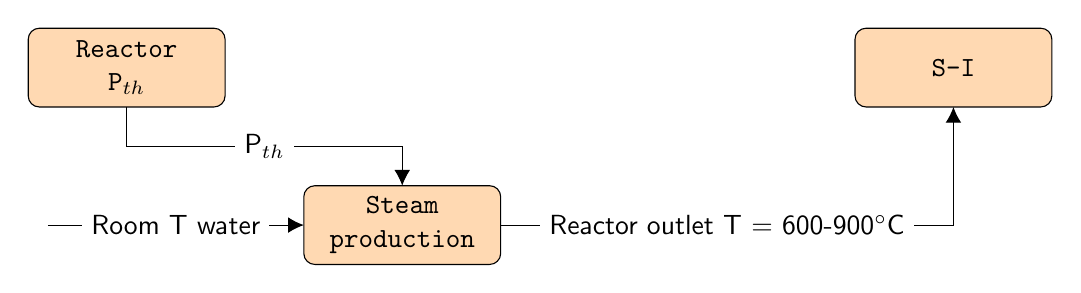
\begin{tikzpicture}[node distance=3cm,
    every node/.style={fill=white, font=\sffamily}, align=center]
  % Specification of nodes (position, etc.)

  \node (reactor)	[process] {Reactor\\P$_{th}$};
  \node (steam2)	[process, below of=reactor, yshift=1.cm, xshift=3.5cm] {Steam\\production};
  \node (si)		[process, right of=reactor, xshift=7.5cm] {S-I};

  \draw[->]			(reactor) ++(0.,-0.5)-- ++(0.,-0.5)-- node[midway] {P$_{th}$} ++(3.5,0.)-- ++(0.,-.5);

  \draw[->]			(steam2) ++(-4.5,0)-- node[midway] {Room T water} ++(3.25,0);
  \draw[->]			(steam2) ++(1.25,0)-- node[midway] {Reactor outlet T = 600-900$^{\circ}$C}++(5.75,0)-- ++(0,1.5);

  \end{tikzpicture}
\end{document}